% !TeX program = xelatex
\documentclass{common/resume}

\usepackage{xeCJK}
\usepackage{graphicx}
\usepackage{tabularx}
\usepackage{array}
\usepackage{ragged2e}
\usepackage{enumitem}        % 提供 \setlist
\usepackage{titlesec}        % 提供 \titleformat 和 \titlespacing
\graphicspath{{assets/}}
\geometry{a4paper,left=0.44in,right=0.44in,top=0.18in,bottom=0.34in,nohead}
\urlstyle{same}

\IfFontExistsTF{Times New Roman}{\setmainfont{Times New Roman}}{\setmainfont{Latin Modern Roman}}
\IfFontExistsTF{SimSun}{\setCJKmainfont[AutoFakeBold=2.0]{SimSun}}{\IfFontExistsTF{NSimSun}{\setCJKmainfont[AutoFakeBold=2.0]{NSimSun}}{\IfFontExistsTF{FandolSong}{\setCJKmainfont{FandolSong}}{}}}
\IfFontExistsTF{Times New Roman}{\setsansfont{Times New Roman}}{}

\definecolor{ResumeBlue}{HTML}{436879}
\definecolor{ResumeGold}{HTML}{B9995A}
\definecolor{LineGray}{HTML}{6F8790}
\definecolor{TextGray}{HTML}{222222}
\hypersetup{hidelinks}
\setlength{\parindent}{0pt}
\setlength{\parskip}{0.04em}
\renewcommand{\arraystretch}{1.00}
\setlist[itemize]{leftmargin=1.12em,itemsep=0.02em,topsep=0.02em,parsep=0pt,partopsep=0pt}

\titleformat{\section}{}{}{0pt}{}
\titlespacing*{\section}{0pt}{0.45em}{0.25em}

\newcommand{\slashSep}{\hspace{0.25em}\textcolor{LineGray}{|}\hspace{0.25em}}
\newcommand{\sectionBar}[1]{%
  \vspace{0.24em}%
  \noindent\colorbox{ResumeBlue}{\makebox[2.30cm][l]{\strut\hspace{0.32em}\textcolor{white}{\bfseries\small #1}}}%
  \hspace{0.12em}\textcolor{LineGray}{\rule[0.45ex]{0.74\linewidth}{0.45pt}}%
  \vspace{0.06em}\par
}
\newcommand{\projectTitle}[3]{%
  \vspace{0.12em}%
  \noindent\begin{tabularx}{\linewidth}{@{}>{\bfseries}X r@{}}
    #1 & {\small #2}\\[-0.10em]
  \end{tabularx}
  {\small #3}\par
  \vspace{0.00em}\par
}
\newcommand{\centerProjectTitle}[3]{%
  \vspace{0.12em}%
  \noindent\begin{tabularx}{\linewidth}{@{}p{3cm}>{\centering\arraybackslash\bfseries}X>{\raggedleft\arraybackslash}p{3cm}@{}}
    & #1 & {\small #2}\\[-0.10em]
  \end{tabularx}
  {\small #3}\par
  \vspace{0.00em}\par
}
\newcommand{\subHead}[1]{\vspace{0.04em}\noindent\textbf{#1：}}
\newcommand{\tech}[1]{\textbf{技术栈：}#1\par}
\newcommand{\tightItem}[1]{\item #1}
\renewcommand{\roleLine}[3]{%    % 改回 \renewcommand，因为文档类已定义
  \noindent\begin{tabularx}{\linewidth}{@{}>{\bfseries}X r@{}}
  #1 & #2\\[-0.15em]
  \end{tabularx}
  {\small #3}\par
}

\begin{document}
\fontsize{9pt}{10.8pt}\selectfont
\color{TextGray}

\begin{tabularx}{\linewidth}{@{}X@{\hspace{0.25cm}}>{\raggedleft\arraybackslash}m{3.04cm}@{}}
\begin{minipage}[c][4.00cm][t]{\linewidth}
  \vspace{0.10cm}
  \noindent\makebox[\linewidth][l]{%
    
\includegraphics[height=1.50cm]{university_logo.png}%
    \hspace{0.62cm}%
    
\includegraphics[height=1.50cm]{zzlab.png}%
    \hspace{0.62cm}%
    
\includegraphics[height=1.50cm]{rm_logo.jpg}%
  }\par
  \vfill
  \noindent\raisebox{-0.50cm}[0pt][0pt]{%
    \begin{minipage}[b]{\linewidth}
      {\fontsize{21pt}{23pt}\selectfont\bfseries 韩竣成}\quad
      {\fontsize{10.2pt}{11.6pt}\selectfont 机器人运控 \slashSep 硬件全栈 \slashSep 嵌入式软件 \slashSep 结构设计}\par
      \vspace{0.40em}
      {\fontsize{9.6pt}{11.0pt}\selectfont 电话：18926467193 \quad 邮箱：\href{mailto:2856463157@qq.com}{2856463157@qq.com} / \href{mailto:h4a6n@outlook.com}{h4a6n@outlook.com}}\par
      \vspace{0.40em}
      {\fontsize{9.6pt}{11.0pt}\selectfont 个人网站：\href{https://hjc78big.top}{https://hjc78big.top}}\par
      \vspace{0.40em}
      {\fontsize{9.6pt}{11.0pt}\selectfont Github：\href{https://github.com/NHK-DOT}{https://github.com/NHK-DOT}}\par
      \vspace{0.06cm}
    \end{minipage}%
  }
\end{minipage}
&
\begin{minipage}[c][4.00cm][c]{3.04cm}
  \centering\fboxsep=0pt\fcolorbox{ResumeBlue}{white}{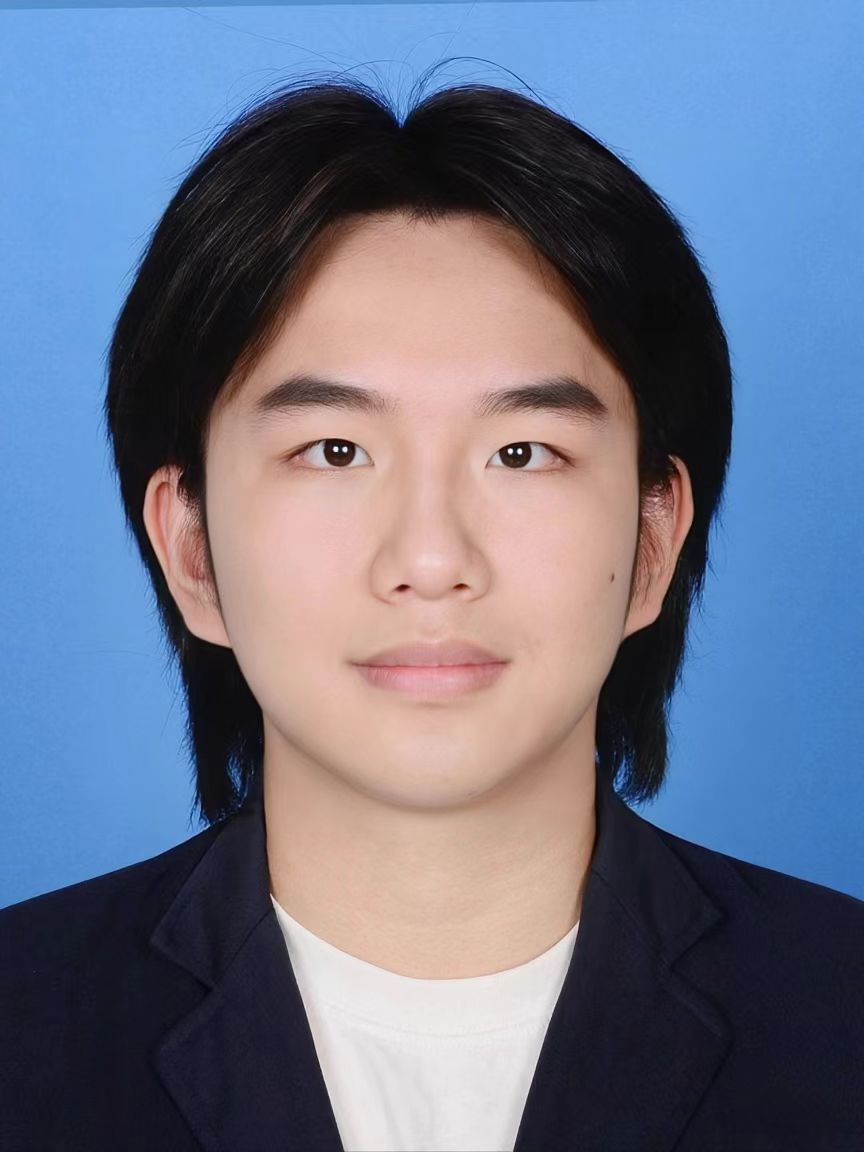
\includegraphics[width=4.00cm,height=4.00cm,keepaspectratio]{photo.jpg}}
\end{minipage}
\end{tabularx}

\vspace{0.02em}
\noindent\textcolor{ResumeBlue}{\rule{0.58\linewidth}{2.8pt}}\textcolor{ResumeGold}{\rule{0.42\linewidth}{2.8pt}}

\sectionBar{教育背景}
\roleLine{河海大学｜人工智能与自动化学院｜自动化本科}{2024.09 -- 预计 2028.06}{主修自动控制原理、数字电路、模拟电路、信号与系统、电机与拖动、FPGA、微机原理等课程。}
\vspace{0.40em}
\roleLine{河海大学智泽实验室｜领队}{2025.09 -- 至今}{负责机器人方向项目组织、项目文档与服务器维护，参与机械结构设计、电机 FOC 控制、嵌入式 PCB layout、\\视觉识别与感知、ROS/导航链路和实机调试；负责新成员招新培训、团队协同管理及日常经费审批报销。}
\vspace{0.40em}
\roleLine{RoboMaster 战队｜机械队员}{2025.11 -- 至今}{负责机械结构与电控联调，参与执行机构设计、零件制造装配、结构改动验证和实机测试维护。}

\sectionBar{项目经历}
\centerProjectTitle{78arm：无人机机械臂自主抓取}{2026 嵌赛国二}{项目队长；负责机械臂结构设计、运动学建模、视觉感知部署、系统集成与实机调试}
\subHead{项目概述}
\begin{itemize}
  \tightItem{\textbf{任务目标：}设计并实现无人机挂载三自由度 Delta 并联机械臂的空中自主抓取系统，贯通机械结构与硬件、视觉感知、运动规划、飞控通信和执行器控制，完成起飞、UWB 远距离接近、视觉精确定位、空中抓取、返航投放的全流程。}
\end{itemize}
\subHead{系统架构与任务链路}
\begin{itemize}
  \tightItem{\textbf{双主控解耦：}飞控运行 ArduPilot 固件并通过串口连接 STM32MP257；MP257 作为通信与控制核心，负责 ROS 2 状态机、UWB 信号处理、MAVROS 飞控指令和机械臂执行器驱动。Jetson Xavier NX 通过有线私有局域网与 MP257 双向通信，仅承担视觉推理与抓取观测，结果经 ROS 2 回传后由 MP257 统一决策。}
  \tightItem{\textbf{任务切换判据：}UWB AoA 将无人机引导至目标附近，进入约 10 cm 半径区域后切换视觉定位；目标置信度与位姿达到阈值时触发下降，电磁铁负载变化引起的电流跃升作为抓取成功判据，并由状态机触发机械臂收回、返航与投放。}
\end{itemize}
\subHead{视觉感知与图像处理}
\begin{itemize}
  \tightItem{\textbf{模型部署：}在 Jetson Xavier NX 上部署 YOLOv8，采用 TensorRT INT8 PTQ 量化，在保持目标识别效果的同时将推理帧率由 37 fps 提升至 45 fps，实现铁质扳手目标的实时识别。}
  \tightItem{\textbf{相机链路优化：}针对 IMX219 鱼眼相机 3K 原画幅最高 21 fps 的限制，修改传感器驱动寄存器开启硬件 binning，调整 V4L2 动态帧率控制、ISP pipeline 与 DMA 缓冲区；将软件降采样1080p 输出提升至 45 fps，同时保留原3K视场角并匹配 Jetson 载板 15 针 MIPI CSI-2 传输。针对 YUY2/YUYV 未压缩流带宽占用高的问题，优先协商 MJPG，驱动侧解码为 RGB24 后进入 OpenCV。}
  \tightItem{\textbf{检测与跟踪：}对鱼眼图像执行降采样、灰度化、阈值/二值化预处理以抑制地面反光；在检测框周围扩展 25\% 区域作为动态 ROI，下一帧优先在 ROI 内推理，置信度不足时回退全局检测，并用卡尔曼滤波平滑目标位置，降低全局推理负载。完成底座鱼眼 AprilTag 检测、眼在手手眼标定与 XYZ 偏置输出，为 MP257 提供抓取位姿输入。}
\end{itemize}
\subHead{机械臂运控与轨迹规划}
\begin{itemize}
  \tightItem{\textbf{上层 A* 路径规划：}STM32MP257 接收视觉侧回传的目标偏置与抓取位姿，以机械臂当前末端位置为起点、目标抓取点为终点；A* 在工作空间遍历结果与软限位约束形成的可达区域内搜索路径，将越界点和两连杆共线的奇异区域排除，输出可执行的 waypoint 序列。}
  \tightItem{\textbf{中层轨迹生成：}对 A* 输出的 waypoint 执行线性时间插补与梯形速度规划，以 200 Hz 生成末端参考轨迹；通过 Delta FK/IK 和三路主动臂角度计算将笛卡尔轨迹转换为关节目标，建立 LX-225 总线舵机 0--1000 raw 位置与 0--360$^\circ$ 关节角的映射，并以 500 raw 作为上电中位。}
  \tightItem{\textbf{下层闭环跟踪：}采用 LQR 跟踪中层关节期望轨迹，融合视觉偏置、末端 AprilTag/IMU 与舵机编码值，经卡尔曼滤波修正观测噪声和执行误差，形成规划—执行闭环。}
  \tightItem{\textbf{工作空间与调试：}基于已采集工作空间设置软限位，并以 8BitDo 手柄映射 XYZ 三轴速度和电磁铁选通，完成工作空间标定、路径遥操验证与自主抓取联调。}
\end{itemize}
\subHead{机械设计、制造与硬件系统}
\begin{itemize}
  \tightItem{\textbf{结构设计：}自主设计 T600 碳纤中心板与 2 mm 厚碳纤维管机臂，以及 CNC 6061 铝合金关节、T300 碳纤维臂管和 FDM PA6CF/PLA 结构件组成的 Delta 机械臂；基于 SolidWorks 完成 40 余个零件建模、装配、运动学仿真和关节有限元静力分析，并对关键件进行受拉压剪校核与轻量化设计。}
  \tightItem{\textbf{电源与执行器：}设计制作 3 套分电降压 DC--DC BUCK 电源板及 STM32F103 舵机驱动板，完成嘉立创原理图/PCB、制板、焊接、固件编写与烧录；使用 LX-225 总线舵机驱动 Delta 机构，末端 12 V 电磁铁由 ESP8266 继电器控制并作为 ROS 2 节点与主控通信。}
  \tightItem{\textbf{迭代与可靠性：}完成四轮装配迭代，通过预留约 10\% 公差、调整 FDM 打印流量和保温措施解决热变形引起的过盈干涉，重新设计折叠起落架规避运动空间冲突；针对重心偏离、飞控共振和起落架干涉分别调整电池/机械臂布局、增加减震板并优化承力结构。}
\end{itemize}
\projectTitle{智慧社区视觉导航小车}{人工智能精英算法大赛国二}{项目队长；负责 ROS、视觉小车、运控、建图导航与路径规划}
\begin{itemize}
  \tightItem{基于 ROS/catkin 工作区组织相机采集、视觉检测、路径与航点导航、激光雷达代价地图和 RViz/IMU 工具；项目目录包含多个 ONNX 检测模型与对应识别节点。}
  \tightItem{围绕智慧社区任务整合目标检测、地图导航和移动底盘控制链路，形成可继续整理为公开仓库的工程材料。}
\end{itemize}
\sectionBar{获奖经历}
\begin{itemize}
  \item 人工智能精英算法大赛智慧社区国二｜队长｜GitHub：\href{https://github.com/NHK-DOT/roscar-second}{\nolinkurl{https://github.com/NHK-DOT/roscar-second}}
  \item 嵌入式竞赛国二｜队长｜GitHub：\href{https://github.com/NHK-DOT/delta_on_quadrotorUAV}{\nolinkurl{https://github.com/NHK-DOT/delta_on_quadrotorUAV}}
  \item 物联网杯省二｜队长｜GitHub：\href{https://github.com/NHK-DOT/Waveshare_PixelMatrixStudio}{\nolinkurl{https://github.com/NHK-DOT/Waveshare_PixelMatrixStudio}}
  \item MCM/ICM 美赛 H 奖｜队长｜GitHub：\href{https://github.com/NHK-DOT/ms-H}{\nolinkurl{https://github.com/NHK-DOT/ms-H}}
  \item 服务外包大赛国三｜队长｜GitHub：\href{https://github.com/NHK-DOT/service_outsourcing}{\nolinkurl{https://github.com/NHK-DOT/service_outsourcing}}
\end{itemize}

\sectionBar{技术栈}
\begin{itemize}
  \item \textbf{机器人/运动控制：} 运动学 (FK/IK)、轨迹规划 (G-code 解析、线性插值、A*、Dijkstra)、
        控制算法 (PID、LQR)、移动抓取与导航 (ROS Navigation、MoveIt、代价地图)、
        多传感器融合 (UWB/AOA、IMU、AprilTag)、舵机/执行器控制。
  \item \textbf{计算机视觉：} OpenCV、YOLO (检测/部署)、AprilTag 位姿估计、相机标定、
        图像流处理 (MJPG/YUYV/RGB24)、特征工程 (降采样、二值化、滤波)。
  \item \textbf{嵌入式系统：} 传感器固件适配 (IMX219、摄像头 ISP 调试)、内核配置与设备树裁剪、
        RTOS 了解 (FreeRTOS/RT-Thread)、
        通信协议 (I2C、SPI、CAN、UART、USB)、
        MCU/MPU 平台 (STM32、ESP32、树莓派、Jetson) 开发与部署。
  \item \textbf{硬件/PCB 设计：} 多层板 PCB Layout (Altium Designer、嘉立创制板)、
        焊接调试、FPGA 应用 (图像处理加速、FOC 电机驱动)、
        传感器接口电路、系统电源方案设计。
  \item \textbf{机械/结构：} 结构设计 (SolidWorks/Fusion 360)、3D 打印/CNC 制造装配、
        执行机构开发 (Delta 机械臂、夹爪)、传感器固定件设计、整机联调。
  \item \textbf{工具/语言：} C/C++、Python、Go、Kotlin、CMake、Linux、Git、Docker；
        ROS 1/2、Gazebo、MoveIt、Nav Stack、MAVROS。
\end{itemize}
\end{document}
